\section{Super Resolution}
\subsection{Implementation}

Among all the models we implemented, WaveFace is a special case. Unlike WaveMix and Non-Local Fast Fourier Convolution (NL-FFC), which are pure super-resolution models, WaveFace serves as an image restoration model designed to improve overall image quality. For this reason, we first apply bicubic interpolation to the low-resolution image before processing it through the WaveFace model. This preprocessing step ensures the input meets the model's requirements while maintaining its enhancement capabilities.

For all models, bigger image cost larger computation cost. To address the computational challenges of processing low-resolution images (1020x768), we adopt a patch-based inference strategy. The input image is divided into overlapping patches of size 48×48 pixels, with a stride of 24 pixels along both width and height. This ensures sufficient overlap to mitigate boundary artifacts during reconstruction.

During inference, each patch is processed independently. To  reconstruct the final output, we maintain a weight matrix that tracks the contribution of each pixel across overlapping patches. This allows us to compute a weighted average during the reconstruction phase, ensuring smooth transitions and preserving fine-grained details in the restored image. This approach significantly reduces memory usage while maintaining high-quality restoration results.

\subsection{Metrics}
In this experiment, we perform comparisons among the models based on the metrics shown in the table below.

\begin{table}[H]
\centering
\caption{Comparison of Wavemix, NL-FCC, and WaveFace Models}
\begin{tabular}{lccc}
\hline
\textbf{Metric} & \textbf{Wavemix} & \textbf{WaveFace} & \textbf{NL-FCC} \\
\hline
\textbf{Total params (M)}         & 11.45   & 0.95   & 0.88 \\
\textbf{Trainable params (M)}     & 11.45   & 0.95   & 0.88 \\
\textbf{Model size (MB)}          & 43.71   & 3.61   & 3.36 \\
\textbf{GFLOPs}                   & 52.73   & 0.0002   & 9.53 \\
\hline
\textbf{ITPP (ms)} &       &        &        \\
\quad Min                          & 4.37    & 836.43  & 10.48 \\
\quad Max                          & 18.07    & 935.97  & 12.50 \\
\quad Mean                         & 4.60 ± 0.62 & 869.08 ± 20.76 & 10.92 ± 0.32 \\
\hline
\textbf{ITPI (ms)} &       &        &        \\
\quad Min                          & 3636.18 & 584454.53 & 7364.14 \\
\quad Max                          & 14830.38 & 1232201.07 & 21310.79 \\
\quad Mean                         & $7.10^3$ ± $10^3$ & $10^6$ ± $10^5$ & $10^4$ ± $2.10^3$ \\
\hline
\textbf{Quality Metrics}           &         &         &        \\
\quad PSNR                         & 28.65 ± 5.27 & 29.34 ± 4.24 & 19.80 ± 1.67 \\
\quad SSIM                         & 0.90 ± 0.06 & 0.87 ± 0.07 & 0.64 ± 0.11 \\
\hline
\end{tabular}
\caption*{\textbf{Abbreviations:} \\
ITPP = Inference Time Per Patch \\
ITPI = Inference Time Per Image}
\label{tab:model_comparison}
\end{table}

Table \ref{tab:model_comparison} is conducted by testing 50 random images in validation dataset of Div2K dataset \cite{Chen_2020_CVPR_Workshops}. Each low-resolution image was passed through the models and compared against its corresponding high-resolution version to evaluate the performance, showing the trade-offs between Wavemix, WaveFace, and NL-FCC models. Wavemix is the most computationally intensive, with 11.45 million parameters, a model size of 43.71 MB, and 52.73 GFLOPs while it offers the best balance between inference speed and output quality. It achieves low mean inference time per patch (ITPP) of 4.60 ms and per image (ITPI) of approximately 7000 ms. In contrast, WaveFace is extremely lightweight computationally (only 0.0002 GFLOPs) and has a small model size. However, it suffers from extremely high inference times, making it impractical for real-time applications despite achieving the highest PSNR of 29.34. NL-FCC is more efficient than WaveFace in terms of inference time, with an ITPI of about $10^4$ ms and a small model size of 3.36 MB, but shows significantly lower image quality (PSNR of 19.80 and SSIM of 0.64). Overall, Wavemix offers the best trade-off for scenarios requiring both performance and quality, while WaveFace may suit highly resource-constrained environments where speed is not critical, and NL-FCC serves as a middle-ground option with modest performance across all metrics.

\subsection{Inference}

\begin{figure}[htbp]
    \centering
    \includegraphics[width=0.6\textwidth]{experiment/images/hr_image.png}
    \caption{Region of ground truth image used for inferencing through each model}
    \label{fig:hr_image}
\end{figure}

\begin{figure}[htbp]
    \centering
    % --- Top Row: 3 Images ---
    \begin{minipage}{0.3\textwidth}
        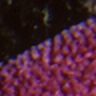
\includegraphics[width=\linewidth]{experiment/images/wavemix_crop.png}
        \caption*{WaveMix}
        \label{fig:1a}
    \end{minipage}
    \hfill
    \begin{minipage}{0.3\textwidth}
        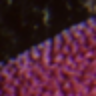
\includegraphics[width=\linewidth]{experiment/images/waveface_crop.png}
        \caption*{WaveFace}
        \label{fig:1b}
    \end{minipage}
    \hfill
    \begin{minipage}{0.3\textwidth}
        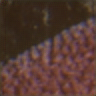
\includegraphics[width=\linewidth]{experiment/images/nlfcc_crop.png}
        \caption*{NL-FCC}
        \label{fig:1c}
    \end{minipage}

    \vspace{0.5cm} % Add vertical spacing between rows

    % --- Bottom Row: 2 Images ---
    \begin{minipage}{0.3\textwidth}
        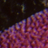
\includegraphics[width=\linewidth]{experiment/images/lr_crop.png}
        \caption*{Low resolution}
        \label{fig:1d}
    \end{minipage}
    \hfill
    \begin{minipage}{0.3\textwidth}
        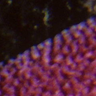
\includegraphics[width=\linewidth]{experiment/images/hr_crop.png}
        \caption*{High resolution}
        \label{fig:1e}
    \end{minipage}

    \caption{Comparison of image, extracted in Figure \ref{fig:hr_image}, passed through each model with ground-truth low resolution and high resolution}
    \label{fig:inference_comparison}
\end{figure}

As shown in Figure \ref{fig:inference_comparison}, most models tend to produce smoother versions of low-resolution images. While WaveMix delivers sharper results, WaveFace appears more blurred. NL-FFC also generates a smoother output, but its color channels exhibit some inconsistencies. This is likely due to imperfections in our implementation compared to the original paper's specifications.

